\chapter{Sensory data distribution}\label{a:dataset}

To investigate some properties of real-world experiments, it is interesting to know how the frequency of segments corresponding to light sources is distribut\-ed. \figref{f:st:distrib_corresp} shows how this distribution is found in the recorded data set. It is interesting to note that light source \textsc{l}\oldstylenums{0} is detected most often; $r1$ segmented \textsc{l}\oldstylenums{0} on the average even more than once a situation. \figref{f:st:distribcontext} shows the distribution of context size frequencies. It should be clear that contexts are not always of equal size within one situation, nor can one observe a normal distribution of set sizes.

Figures \ref{f:st:distribl0} and \ref{f:st:distribl3} show how the data is distributed after segmentation and feature extraction has been applied on the basic data set. The figures show the distributions of features for dimensions (a) \textsc{wl}\oldstylenums{0}, (b) \textsc{wl}\oldstylenums{1}, (c) \textsc{wl}\oldstylenums{2} and (d) \textsc{wl}\oldstylenums{3} after perceiving light sources \textsc{l}\oldstylenums{0} and \textsc{l}\oldstylenums{3}. The x-axes show the intervals between 0 and 1 with step-sizes of 0.1. The lower bound is included in the intervals and the upper bound is not. The last ``interval'' shows the frequency of feature value 1.0. The figures should be read as follows: When a certain sensory channel reads feature value 1.0, this sensory channel corresponds with the light source at the same height (e.g. $sc0$ corresponds with \textsc{l}\oldstylenums{0}). The relative frequency of reading feature value 1.0 for this referent is 1. The relative frequencies of all other sensory channels is distributed on the sensory space. It should be clear that most feature values of other sensory channels read values in the interval $[0.0,0.1\rangle$. 
However, there are more sensory channels that are not directly adjacent. Between 0.1 and 1.0, the distribution is low and not structurally distributed. Hence the data shows no clear laws in the distribution. This indicates the noisy perception of the robots. Noise that cannot directly be simulated.

\begin{figure}[h]
\centering
\subfigure{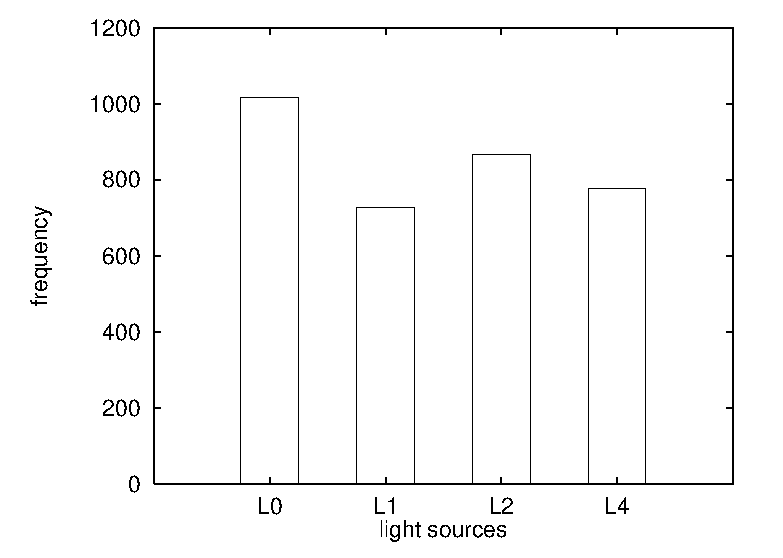
\includegraphics[width=.45\textwidth]{basic//distcorr0.eps}}
\subfigure{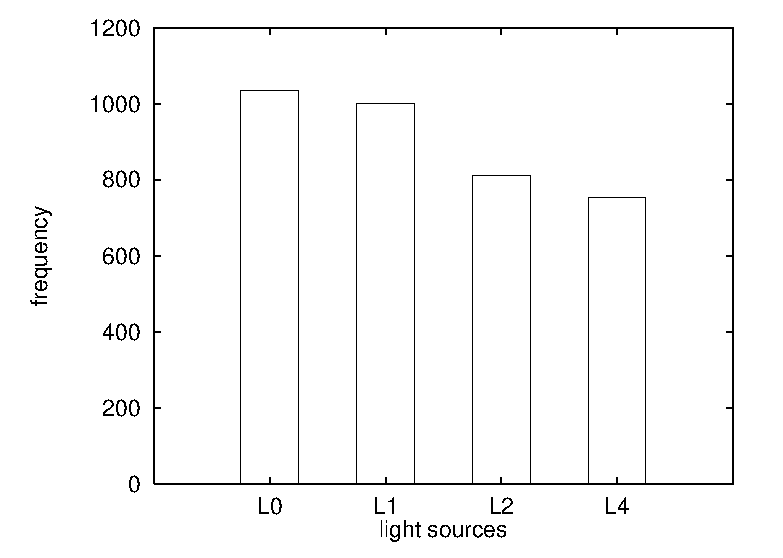
\includegraphics[width=.45\textwidth]{basic//distcorr1.eps}}
\caption{The distribution of the frequency of corresponding segments in the data set for robots $r0$ (a) and $r1$ (b).}
\label{f:st:distrib_corresp}
\end{figure}\enlargethispage{2\baselineskip}

\begin{figure}[h]
\centering
\subfigure{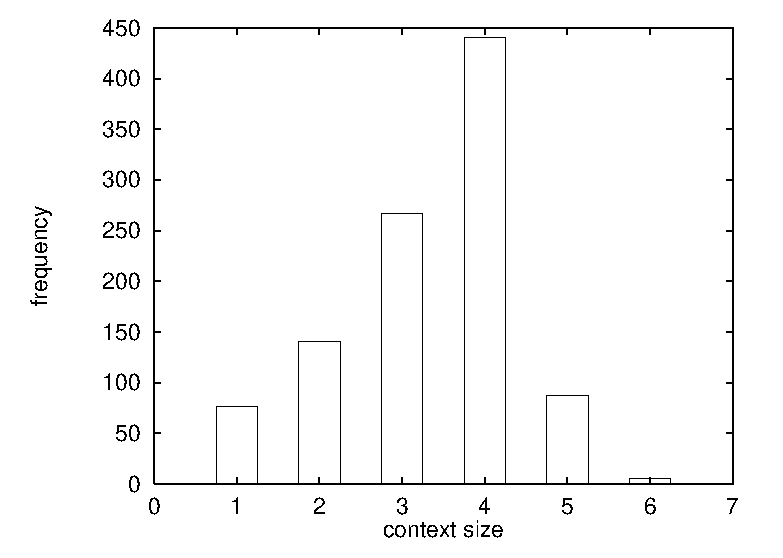
\includegraphics[width=.45\textwidth]{basic//distcont0.eps}}
\subfigure{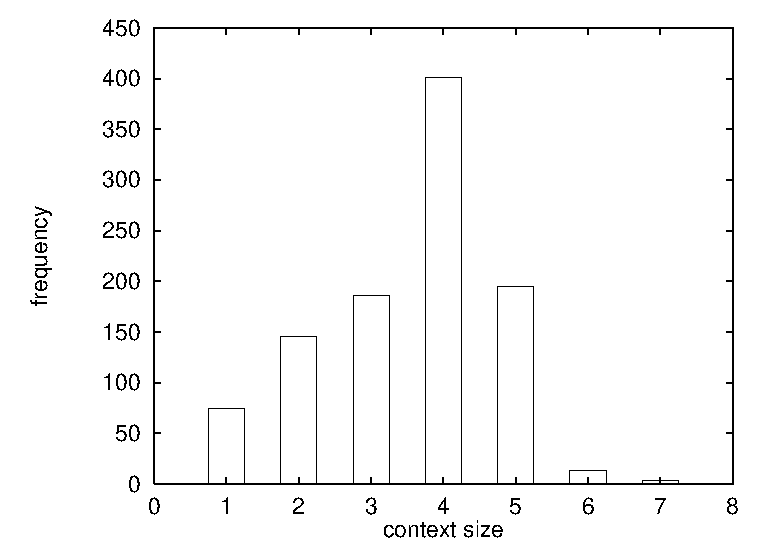
\includegraphics[width=.45\textwidth]{basic//distcont1.eps}}
\caption{The frequency distribution of context sizes of robots $r0$ (a) and $r1$ (b).}
\label{f:st:distribcontext}
\end{figure}

\begin{figure}[h]
\centering
\subfigure[WL0]{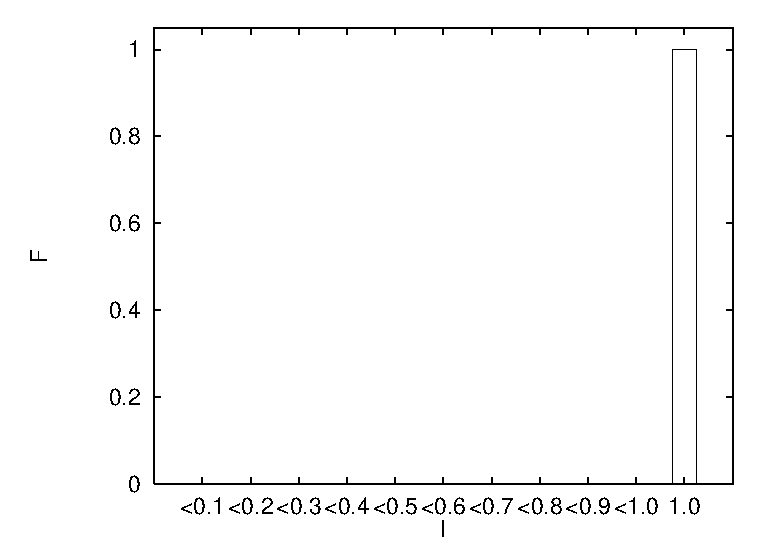
\includegraphics[width=.45\textwidth]{basic//r0l0basis.eps}}
\subfigure[WL1]{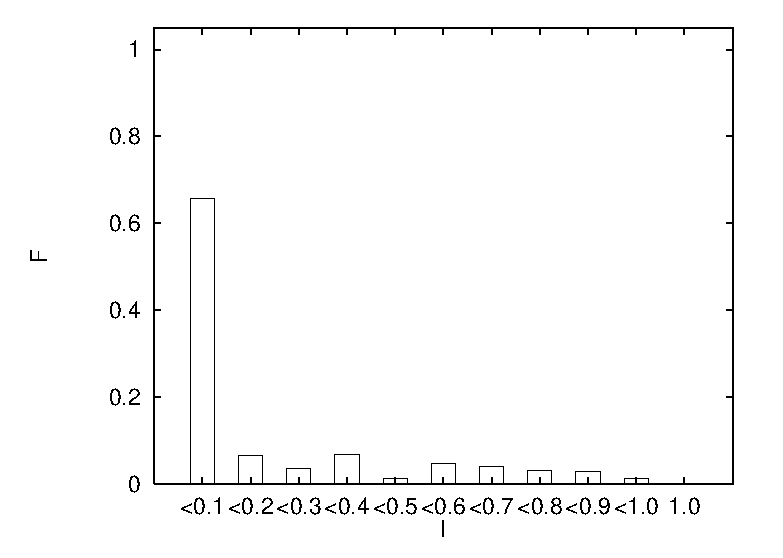
\includegraphics[width=.45\textwidth]{basic//r0l0s1basis.eps}}
\end{figure}
\begin{figure}
\centering
\subfigure[WL2]{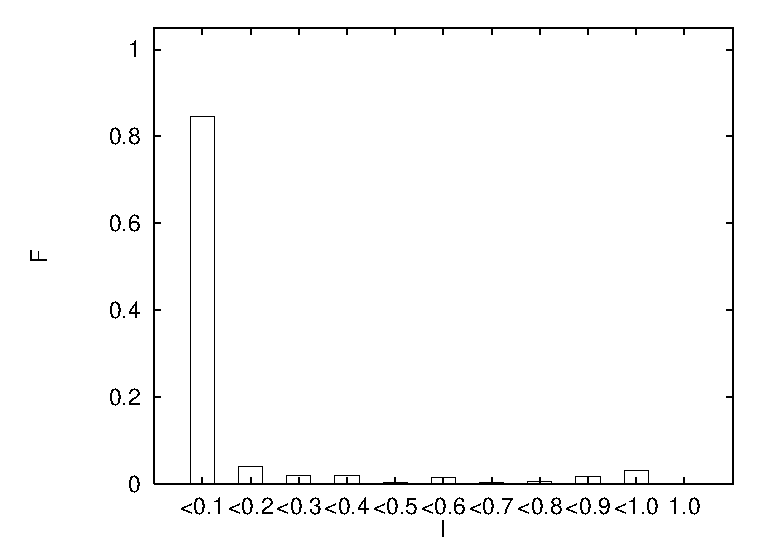
\includegraphics[width=.45\textwidth]{basic//r0l0s2basis.eps}}
\subfigure[WL3]{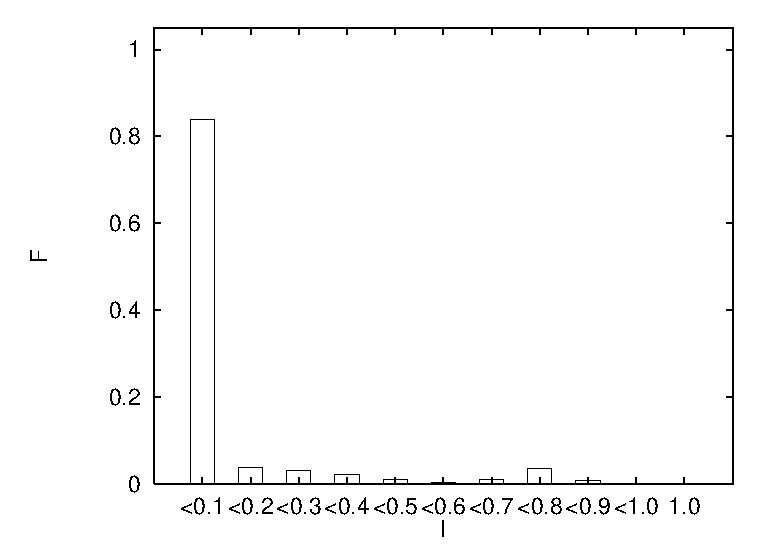
\includegraphics[width=.45\textwidth]{basic//r0l0s3basis.eps}}
\caption{The distribution of feature values observed for light source \textsc{l}\oldstylenums{0}.}
\label{f:st:distribl0}
\end{figure}

\begin{figure}[h]
\centering
\subfigure[WL0]{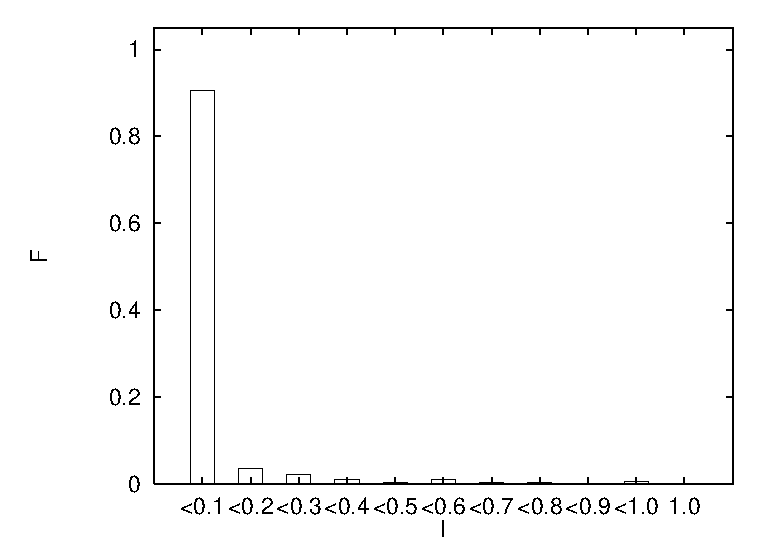
\includegraphics[width=.45\textwidth]{basic//r0l3basis.eps}}
\subfigure[WL1]{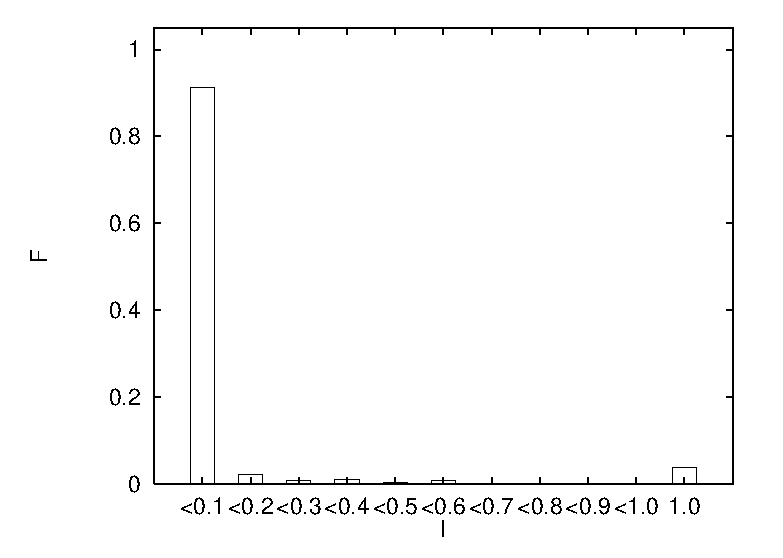
\includegraphics[width=.45\textwidth]{basic//r0l3s1basis.eps}}
\subfigure[WL2]{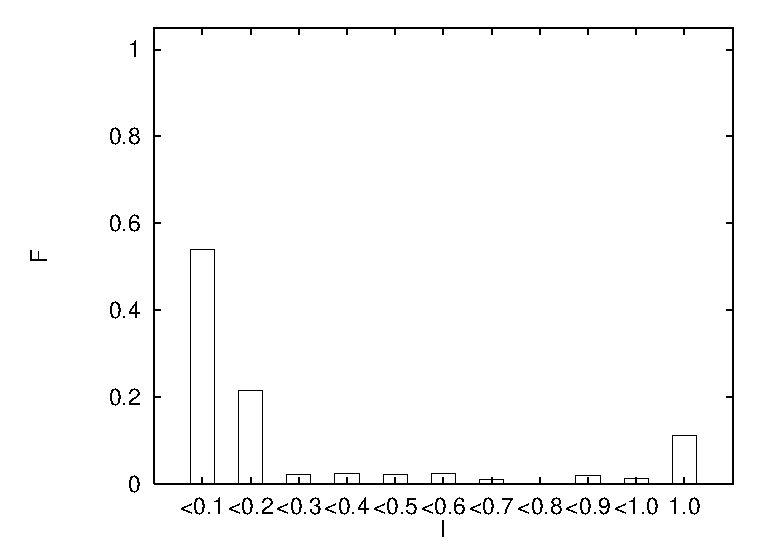
\includegraphics[width=.45\textwidth]{basic//r0l3s2basis.eps}}
\subfigure[WL3]{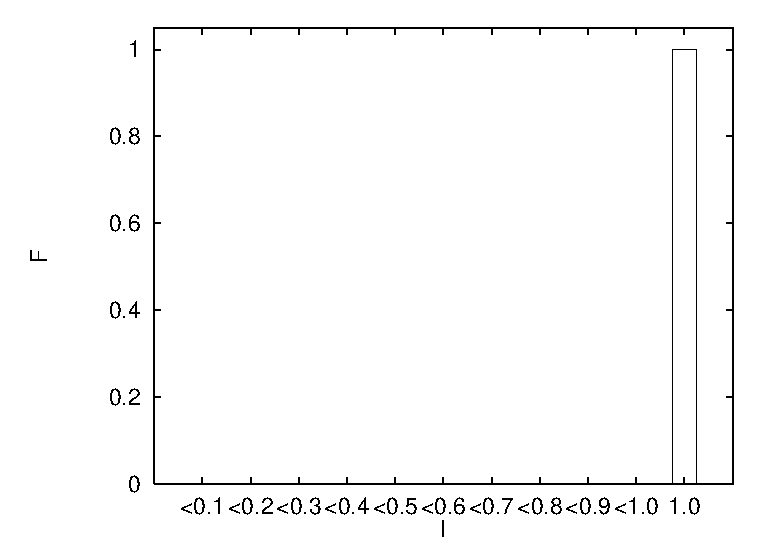
\includegraphics[width=.45\textwidth]{basic//r0l3s3basis.eps}}
\caption{The distribution of feature values observed for light source \textsc{l}\oldstylenums{3}.}
\label{f:st:distribl3}
\end{figure}



